% T402 Architecture Diagram - Standalone TikZ
% Compile with: pdflatex architecture.tex

\documentclass[tikz,border=10pt]{standalone}
\usepackage{tikz}
\usetikzlibrary{arrows.meta, shapes.geometric, positioning, calc, fit, backgrounds, decorations.pathreplacing}
\usepackage{xcolor}

% Define colors
\definecolor{t402blue}{HTML}{3B82F6}
\definecolor{t402green}{HTML}{10B981}
\definecolor{t402purple}{HTML}{8B5CF6}
\definecolor{t402gray}{HTML}{6B7280}
\definecolor{t402orange}{HTML}{F59E0B}

\begin{document}
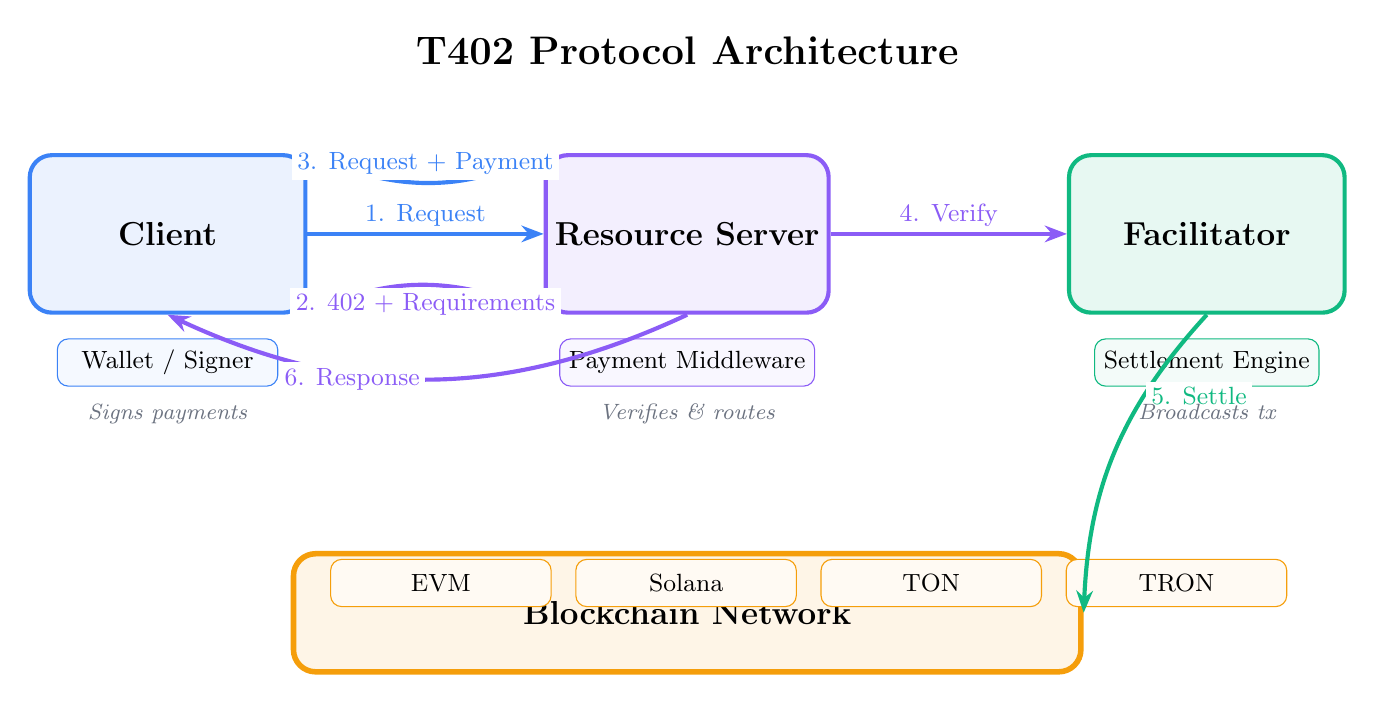
\begin{tikzpicture}[
    node distance=2.5cm and 3cm,
    component/.style={
        rectangle,
        rounded corners=8pt,
        minimum width=3.5cm,
        minimum height=2cm,
        draw=#1,
        line width=1.5pt,
        fill=#1!10,
        font=\bfseries\large
    },
    subcomponent/.style={
        rectangle,
        rounded corners=4pt,
        minimum width=2.8cm,
        minimum height=0.6cm,
        draw=#1,
        fill=#1!5,
        font=\small
    },
    blockchain/.style={
        rectangle,
        rounded corners=8pt,
        minimum width=10cm,
        minimum height=1.5cm,
        draw=t402orange,
        line width=2pt,
        fill=t402orange!10,
        font=\bfseries\large
    },
    arrow/.style={
        ->,
        >={Stealth[length=8pt]},
        line width=1.5pt,
        #1
    },
    label/.style={
        font=\small,
        fill=white,
        inner sep=2pt
    }
]

% Main components
\node[component=t402blue] (client) {Client};
\node[component=t402purple, right=of client] (server) {Resource Server};
\node[component=t402green, right=of server] (facilitator) {Facilitator};

% Subcomponents
\node[subcomponent=t402blue, below=0.3cm of client.south] (wallet) {Wallet / Signer};
\node[subcomponent=t402purple, below=0.3cm of server.south] (middleware) {Payment Middleware};
\node[subcomponent=t402green, below=0.3cm of facilitator.south] (settler) {Settlement Engine};

% Blockchain layer
\node[blockchain, below=3cm of server] (blockchain) {Blockchain Network};

% Blockchain sub-elements
\node[subcomponent=t402orange, below=0.1cm of blockchain.north west, anchor=north west, xshift=0.5cm] (evm) {EVM};
\node[subcomponent=t402orange, right=0.3cm of evm] (solana) {Solana};
\node[subcomponent=t402orange, right=0.3cm of solana] (ton) {TON};
\node[subcomponent=t402orange, right=0.3cm of ton] (tron) {TRON};

% Arrows with labels
\draw[arrow=t402blue] (client) -- node[label, above] {1. Request} (server);
\draw[arrow=t402purple, bend right=25] (server.south west) to node[label, below, pos=0.5] {2. 402 + Requirements} (client.south east);
\draw[arrow=t402blue, bend right=25] (client.north east) to node[label, above, pos=0.5] {3. Request + Payment} (server.north west);
\draw[arrow=t402purple] (server) -- node[label, above] {4. Verify} (facilitator);
\draw[arrow=t402green, bend right=20] (facilitator.south) to node[label, right, pos=0.3] {5. Settle} (blockchain.east);
\draw[arrow=t402purple, bend left=25] (server.south) to node[label, left, pos=0.5] {6. Response} (client.south);

% Annotations
\node[font=\footnotesize\itshape, t402gray, below=0.1cm of wallet] {Signs payments};
\node[font=\footnotesize\itshape, t402gray, below=0.1cm of middleware] {Verifies \& routes};
\node[font=\footnotesize\itshape, t402gray, below=0.1cm of settler] {Broadcasts tx};

% Title
\node[font=\bfseries\Large, above=1cm of server] {T402 Protocol Architecture};

\end{tikzpicture}
\end{document}
